\documentclass{article}
\usepackage{graphicx} % Required for inserting images
\usepackage{caption}
\usepackage{subcaption}
\usepackage{xcolor}
\usepackage{tcolorbox}

\title{ASN2}
\author{William Grimmer, Jack Formato, Victoria Shelton}
\date{October 2024}

\begin{document}

\maketitle

\section{Design}
For our design we chose to do a layered architecture with a three tiered architecture model. It will have the GUI as the top layer, the application as the middle layer and the database as the bottom layer. We chose this as it works well with JavaScript and although MVC is commonly used we felt as if it would be easier to learn and understand layered architecture.

\subsection{Language}
For our language we will use JavaScript as we understand it is one of the premier languages for web applications and has tons of frameworks and libraries that support it such as Node and React. In addition Victoria has also worked with the language before which will help significantly with the learning curve.

\subsection{Frameworks/Libraries}
For our Frameworks and Libraries we will almost certainly use Node.js and React.js. Node.js is what allows for server side JavaScript hosting and will be necessary in order to create a web application. React.js helps to build user interfaces and the front end for web applications and will be very useful. For our testing framework we will be using Jest which is the newest and most common testing framework for JavaScript.

\subsection{Database}

For our Database we will use MySQL. We chose a SQL database over a noSQL version as Will and Jack are familiar with SQL from taking DBMS with Dr. Rocha. For that same reason we will use MySQL as our choice of SQL database as once again we are familiar with it.

\begin{figure}[h]
\centering
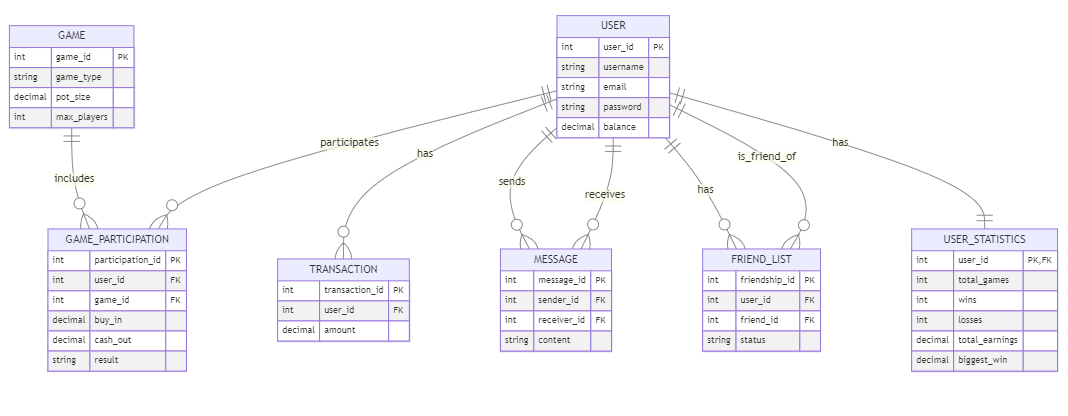
\includegraphics[width=\linewidth]{ERD.png}
\caption{\label{fig:erd}The Entity Relations Diagram for SQL.}
\end{figure}

\newpage
\subsection{coding standards}
For our coding standards we will follow Agile development and work iteratively in coding sprints. The goal is to prioritize working code and not commit anything that covers less than 70\% of test cases. Additionally we will use CamelCase as a naming convention to ensure consistency throughout the code. 


\section{UML}
Figure \ref{fig:uml} is our UML Diagram. This illustrates the class relationships in our project. Users will have Messages and UserStats. We have an Admin class which will extend. Admins, unlike normal Users, will be able to change a User's password. The Game Class has a Host, Players and a Deck. A Player will have a user, in order to add balance and update stats. A deck will be composed of Cards which are dependent on the deck and only exists with it. Players will have a hand, which consists of cards. A game will also have bots. Just like Players, Bots have a hand. These relationships should allow the program to run smoothly and efficiently.

\begin{figure}[h]
\centering
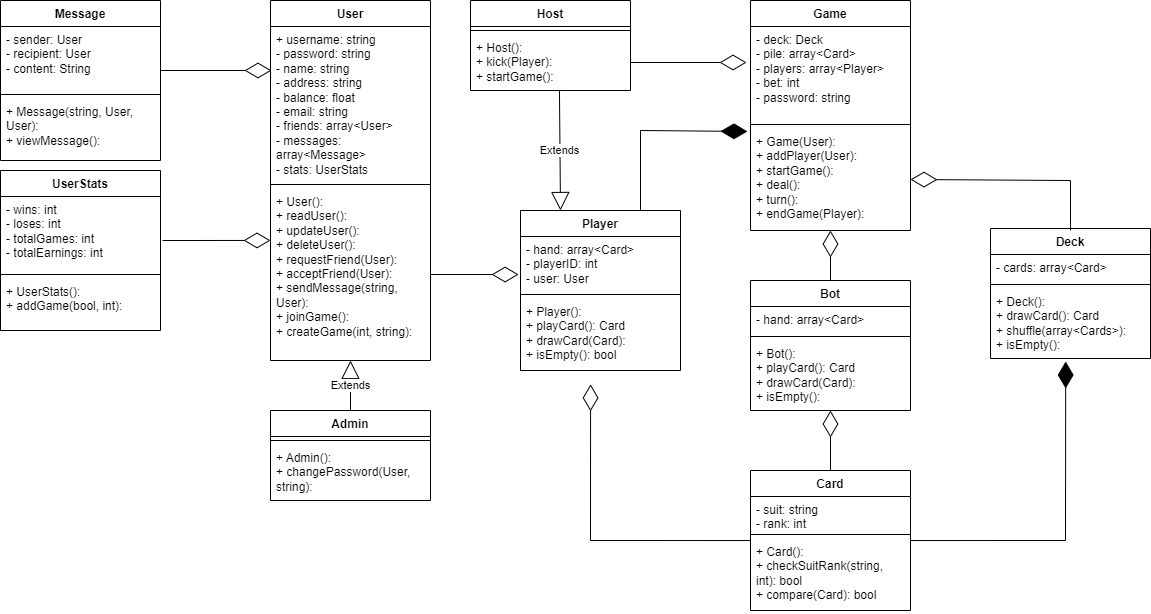
\includegraphics[width=\linewidth]{Crazy8sUML.png}
\caption{\label{fig:uml}High-level OOA UML Class Diagram}
\end{figure}

\section{Website UI Mockup}
\begin{figure}[h]
\centering
\begin{subfigure}{0.5\textwidth}
  \centering
  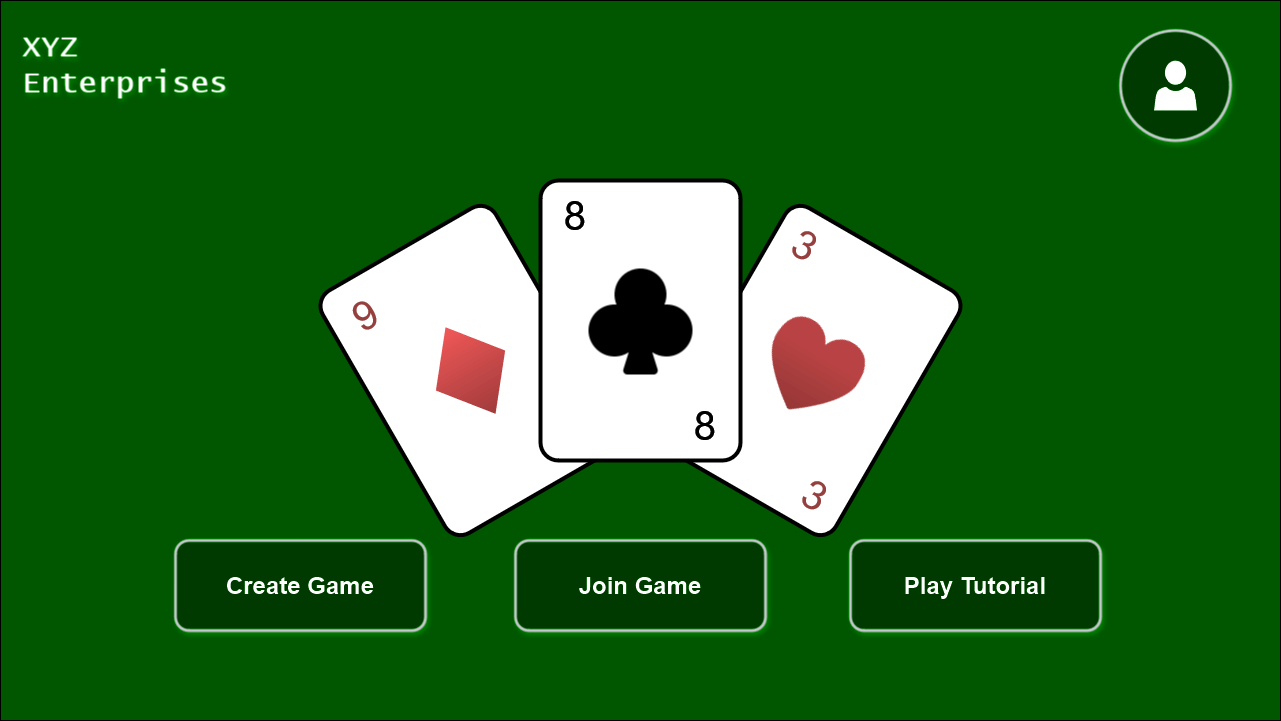
\includegraphics[width=.99\linewidth]{Menu.png}
  \caption{\label{fig:menu}The main menu.}
\end{subfigure}%
\begin{subfigure}{0.5\textwidth}
  \centering
  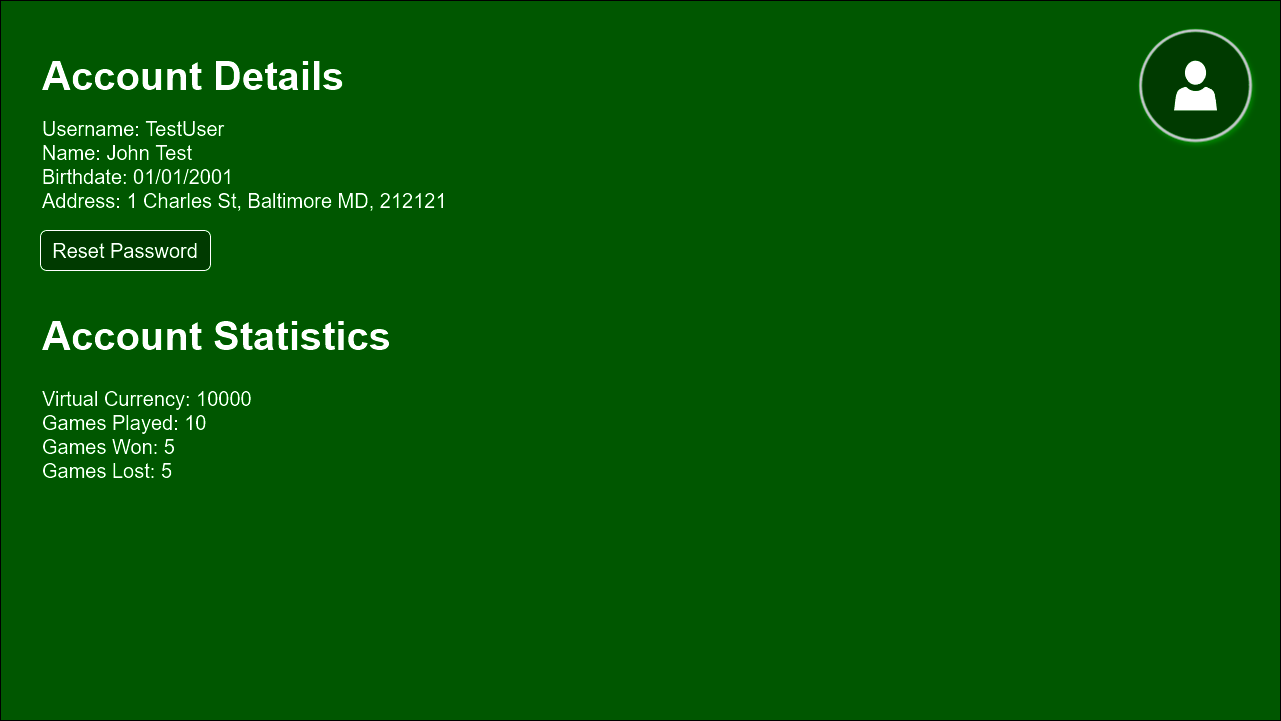
\includegraphics[width=.99\linewidth]{Account.png}
  \caption{\label{fig:account}The account menu.}
\end{subfigure}
\begin{subfigure}{0.5\textwidth}
  \centering
  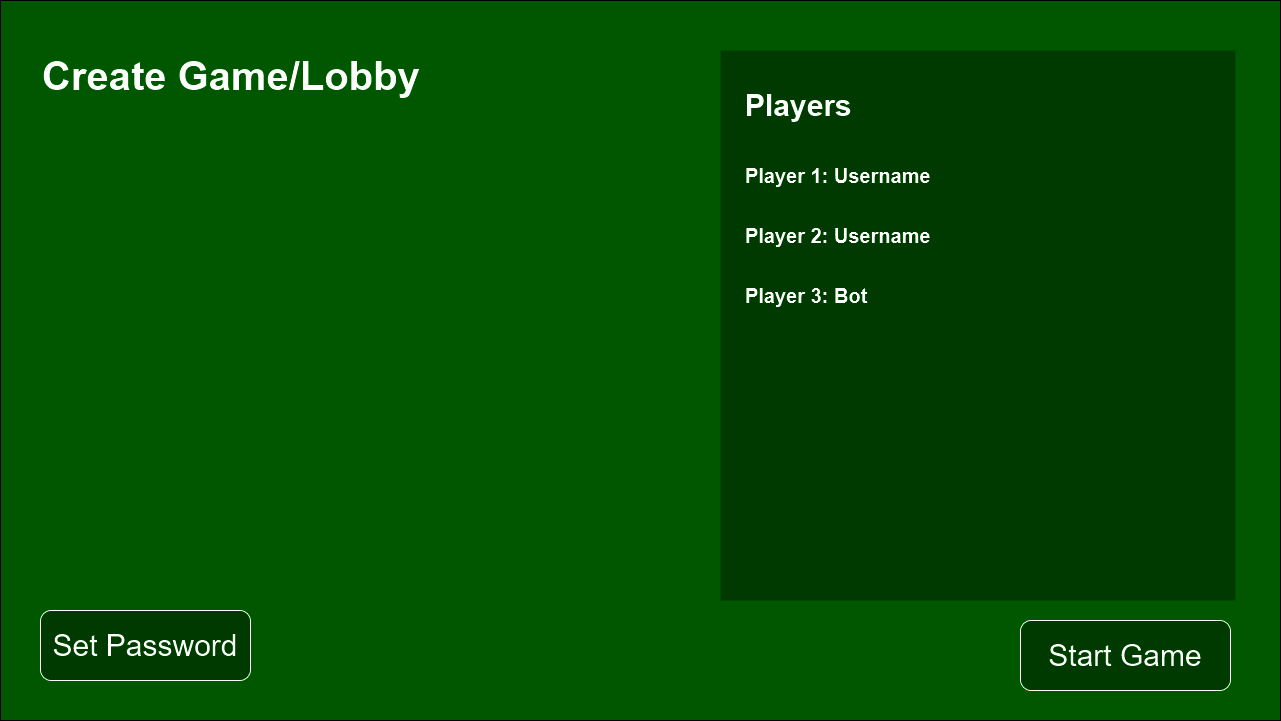
\includegraphics[width=.99\linewidth]{Create.png}
  \caption{\label{fig:create}The create game menu.}
\end{subfigure}%
\begin{subfigure}{0.5\textwidth}
  \centering
  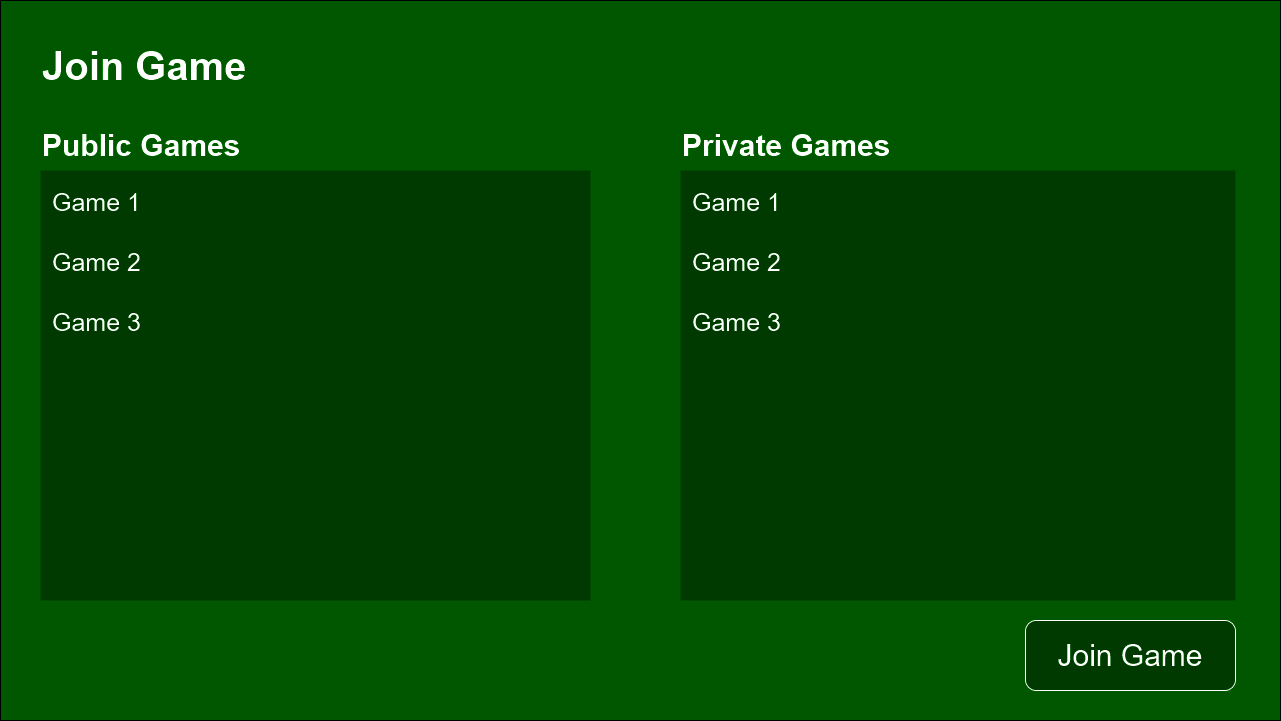
\includegraphics[width=.99\linewidth]{Join.png}
  \caption{\label{fig:join}The join game menu.}
\end{subfigure}
\begin{subfigure}{0.5\textwidth}
  \centering
  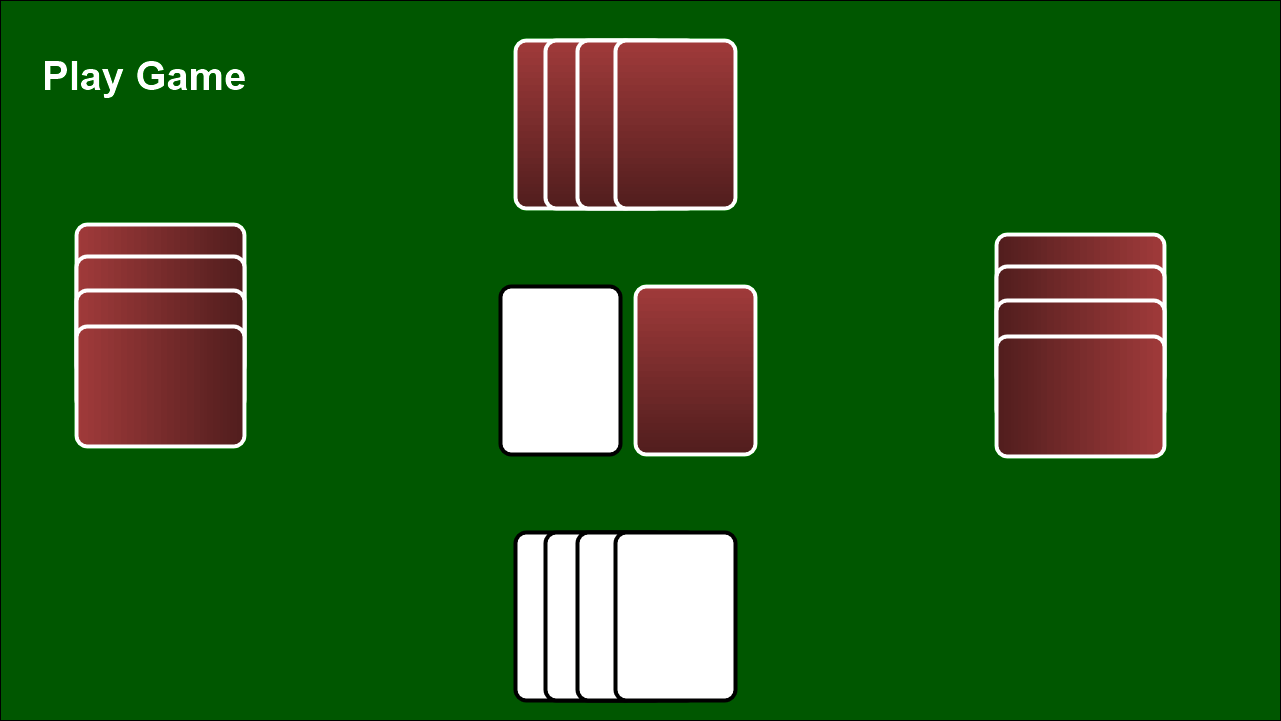
\includegraphics[width=.99\linewidth]{Game.png}
  \caption{\label{fig:game}The game menu.}
\end{subfigure}%
\begin{subfigure}{0.5\textwidth}
  \centering
  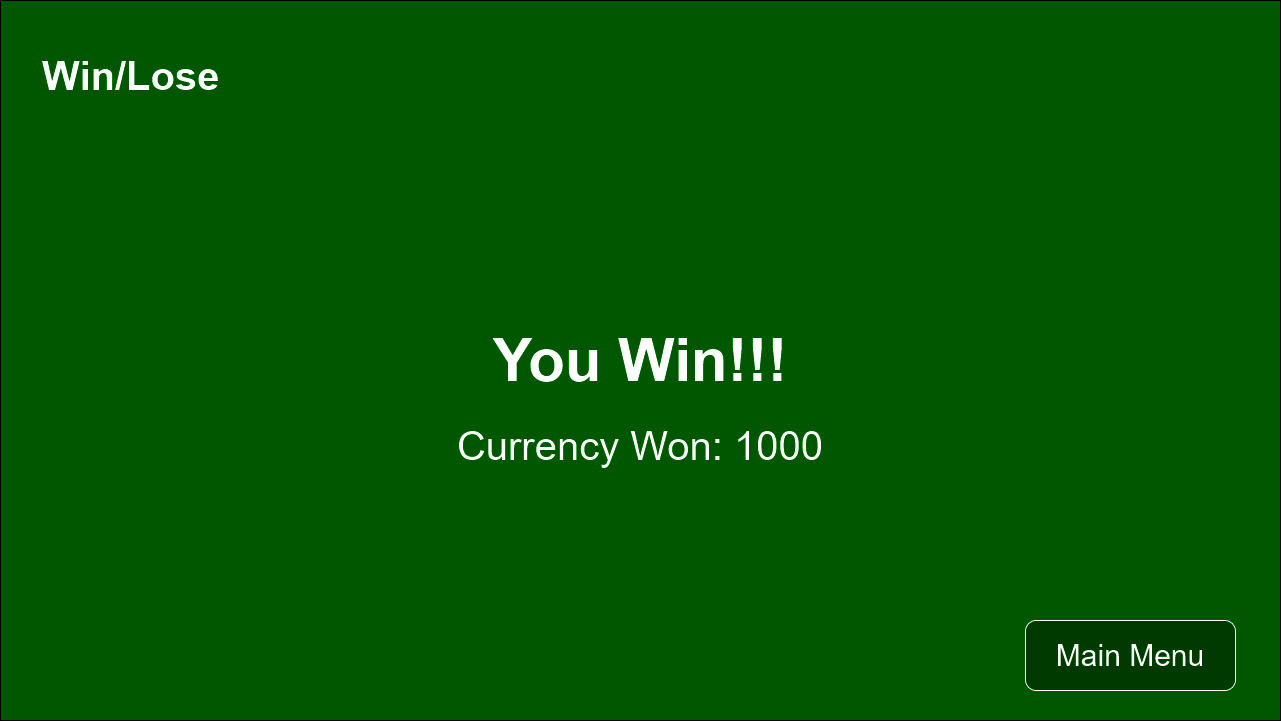
\includegraphics[width=.99\linewidth]{End.png}
  \caption{\label{fig:end}The end screen.}
\end{subfigure}
\end{figure}

The UI for the website should be simple and intuitive. For the main page (see Figure \ref{fig:menu}), the user has four options: create a game, join a game, play the tutorial, or check their account. The account menu page (see Figure \ref{fig:account}) allows users to check their account information and update their password. The create game page in Figure \ref{fig:create} allows users to host a game, set a password, manage players, etc. Players can also join games through the join game page in Figure \ref{fig:join}. When players are in a game, they see the screen in Figure \ref{fig:game}. Lastly, when a game ends, players will see the end screen in Figure \ref{fig:end}, which shows a message based on whether they win or lose and allows them to return to the main screen.

\section{Sprints}

\begin{tcolorbox}[colback=blue!10, colframe=blue, boxrule=0.5mm, sharp corners=south]
\subsection{Sprint Statistics}
\end{tcolorbox}
\begin{table}[h]
\centering
\begin{tabular}{|c|c|c|c|}
\hline
\textbf{Sprint}          & \textbf{Sprint 1} & \textbf{Sprint 2} & \textbf{Sprint 3} \\ \hline
Story Points Done        & 0                 & 18                & 48                \\ \hline
Story Points Remaining   & 69                & 51                & 28                \\ \hline
Story Points Attempted   & 28                & 38                & 28                \\ \hline
Story Points in Backlog  & 41                & 13                & 0                 \\ \hline
Completed Points (Speed) & 28                & 38                & 24                \\ \hline
Team Hours Per Point     & 3.5               & 2                 & 2.3               \\ \hline
\end{tabular}
\end{table}

\subsection{Sprint 1}
\subsubsection{Changes and Slices}
For Sprint 1, we realized that the user story, H0: Create Game, was too large at 13 points. So we decided to split it into H0.1: Create Lobby at 5 points, H0.2: Start Lobby at 5 points, and H0.3: Leave Game at 1 point. This made the task ahead clearer, as it emphasized that the lobby and game were separate pages with different functions.

\subsubsection{User Stories Attempted}
Our team chose to take on a varied array of user stories so that we could build a solid framework for the next sprints. Will worked on the account CRUD-related user stories: A1: Create Account, A2: Update Account, A3: Delete Account, and A4: Check Account. Jack worked on the stories relating to the game system: P1: Play Card and P2: Draw Card. Victoria worked on the UI related stories: H0.1: Create Game and H0.2: Start Lobby. These stories added up to 28 points, out of 72 total points.

\begin{table}[h]
\centering
\begin{tabular}{|c|c|c|c|}
\hline
\textbf{Member} & \textbf{Stories Attempted} & \textbf{Story Points} & \textbf{Hours per Point} \\ \hline
Will     & 4 & 8  & 2 \\ \hline
Victoria & 2 & 10 & 3 \\ \hline
Jack     & 2 & 10 & 3 \\ \hline
Team    & 8 & 28 & 3.5 \\ \hline
\end{tabular}
\end{table}

\subsubsection{Tests}
The summary and graph of the tests done by Jest are shown in figure \ref{fig:test1} and \ref{fig:test2}. Most of the tests succeeded, but one was very tricky to execute, even though the content it was testing worked.

\begin{figure}[h]
\centering
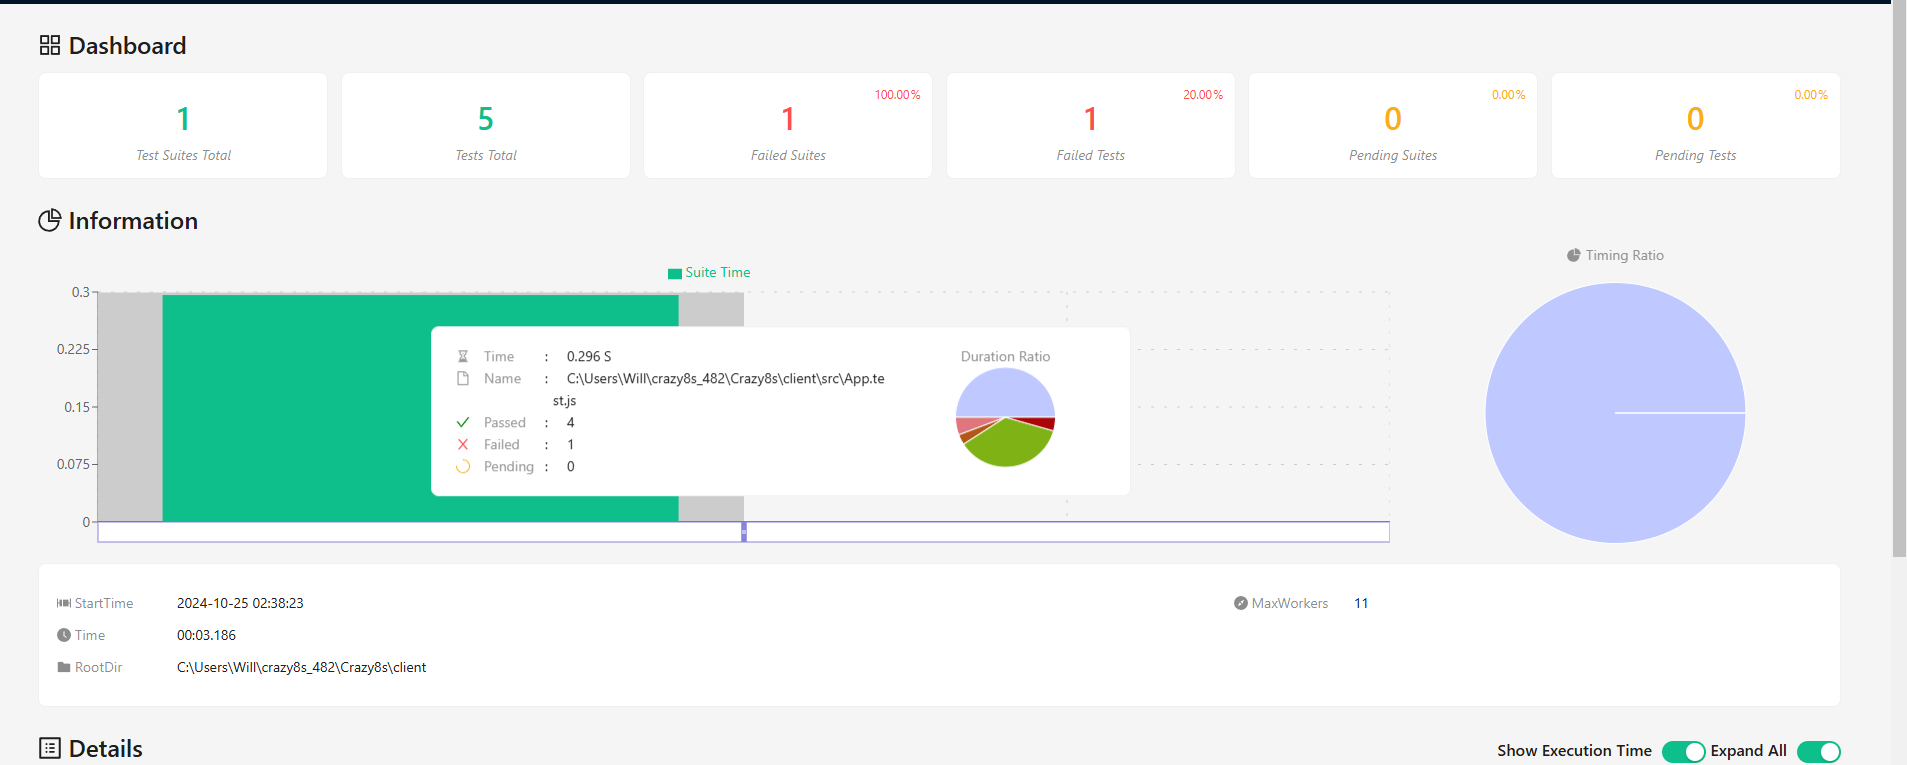
\includegraphics[width=\linewidth]{tests1.png}
\caption{\label{fig:test1}The tests visual summary generated by Jest.}
\end{figure}

\begin{figure}[h]
\centering
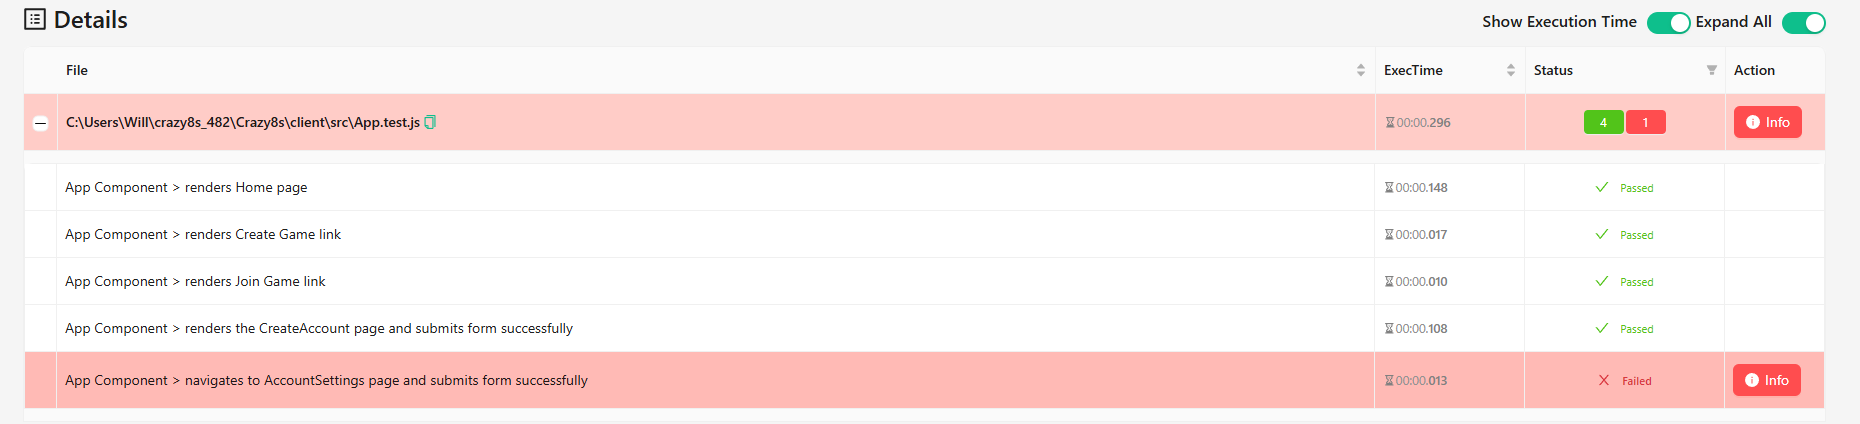
\includegraphics[width=\linewidth]{tests2.png}
\caption{\label{fig:test2}The tests using Jest.}
\end{figure}

\subsection{Sprint 2}

\begin{tcolorbox}[colback=blue!10, colframe=blue, boxrule=0.5mm, sharp corners=south]
\subsection{Retrospective}
Sprint 1 was a good learning experience. We should've started earlier, but struggled too with other work. The biggest issue we had was underestimated the time it took for the initial setup. We also had to learn JavaScript and React syntax for the first time. We also realized that there are no free SQL databases. Due to these issues we will address them by starting earlier and refactoring our database to use Firebase.
\end{tcolorbox}

\subsubsection{Changes and Slices}
For Sprint 2, we did not make any changes or slices.

\subsubsection{User Stories Attempted}

For the second sprint, the team focused on finishing important functionality. Victoria took these stories: View Games, Add Friend, and Accept friend, as well as improving on Create Lobby. Will took Log in, Change Password, Send Message, and Read Message. However, time constraints did not allow for finishing Send Message. Jack did Join Game and Leave Game, as well as finishing Play Card.

\begin{table}[h]
\centering
\begin{tabular}{|c|c|c|c|}
\hline
\textbf{Member} & \textbf{Stories Attempted} & \textbf{Story Points} & \textbf{Hours per Point} \\ \hline
Will     & 3 & 10  & 1.5 \\ \hline
Victoria & 4 & 14 & 2.5 \\ \hline
Jack     & 3 & 14 & 2 \\ \hline
Team    & 10 & 38 & 2 \\ \hline
\end{tabular}
\end{table}

\subsubsection{Tests}
The summary and graph of the tests on the webpages done by Jest are shown in figure \ref{fig:testss2_1} and \ref{fig:testss2_2}. The tests on the classes are shown in \ref{fig:testss2_3}.

\begin{figure}[h]
\centering
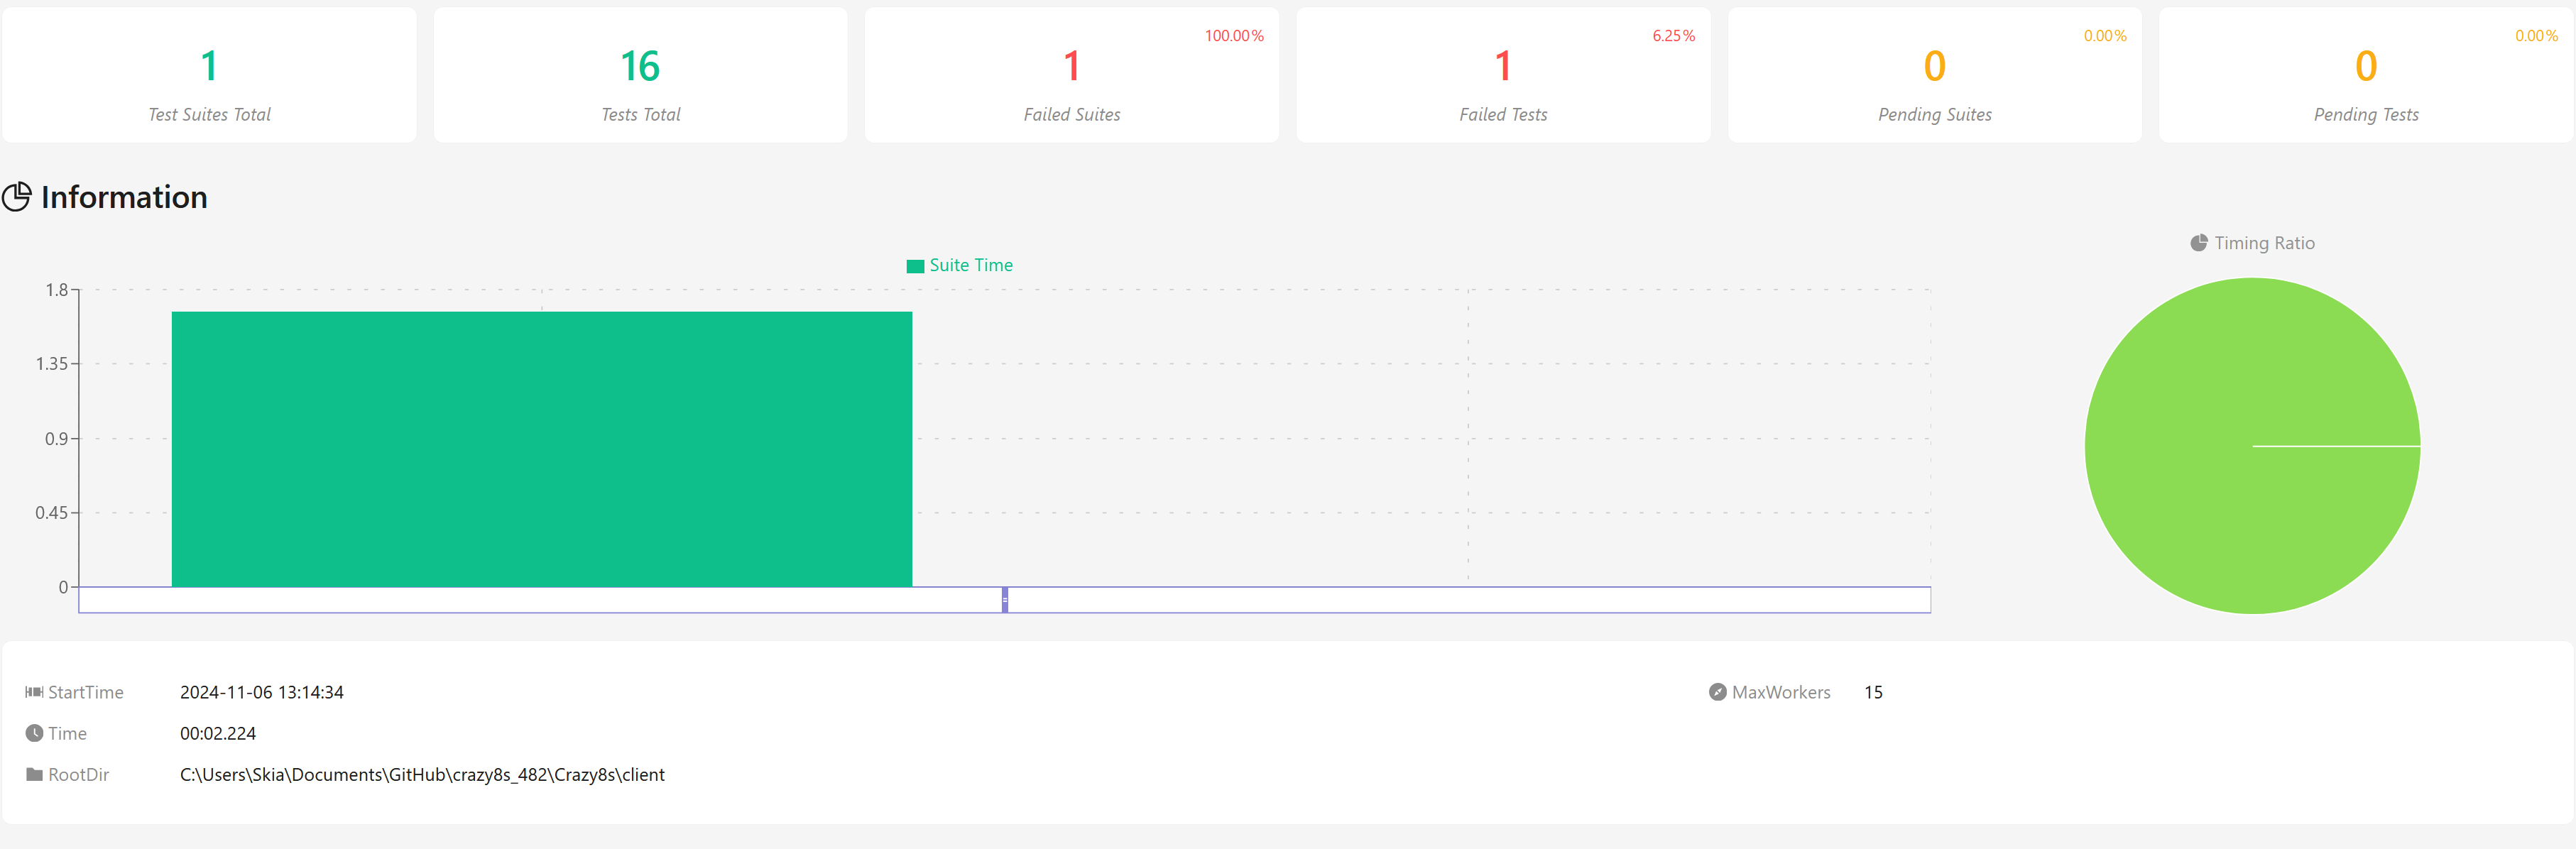
\includegraphics[width=\linewidth]{testss2_1.png}
\caption{\label{fig:testss2_1}The tests visual summary of the webpages generated by Jest.}
\end{figure}

\begin{figure}[h]
\centering
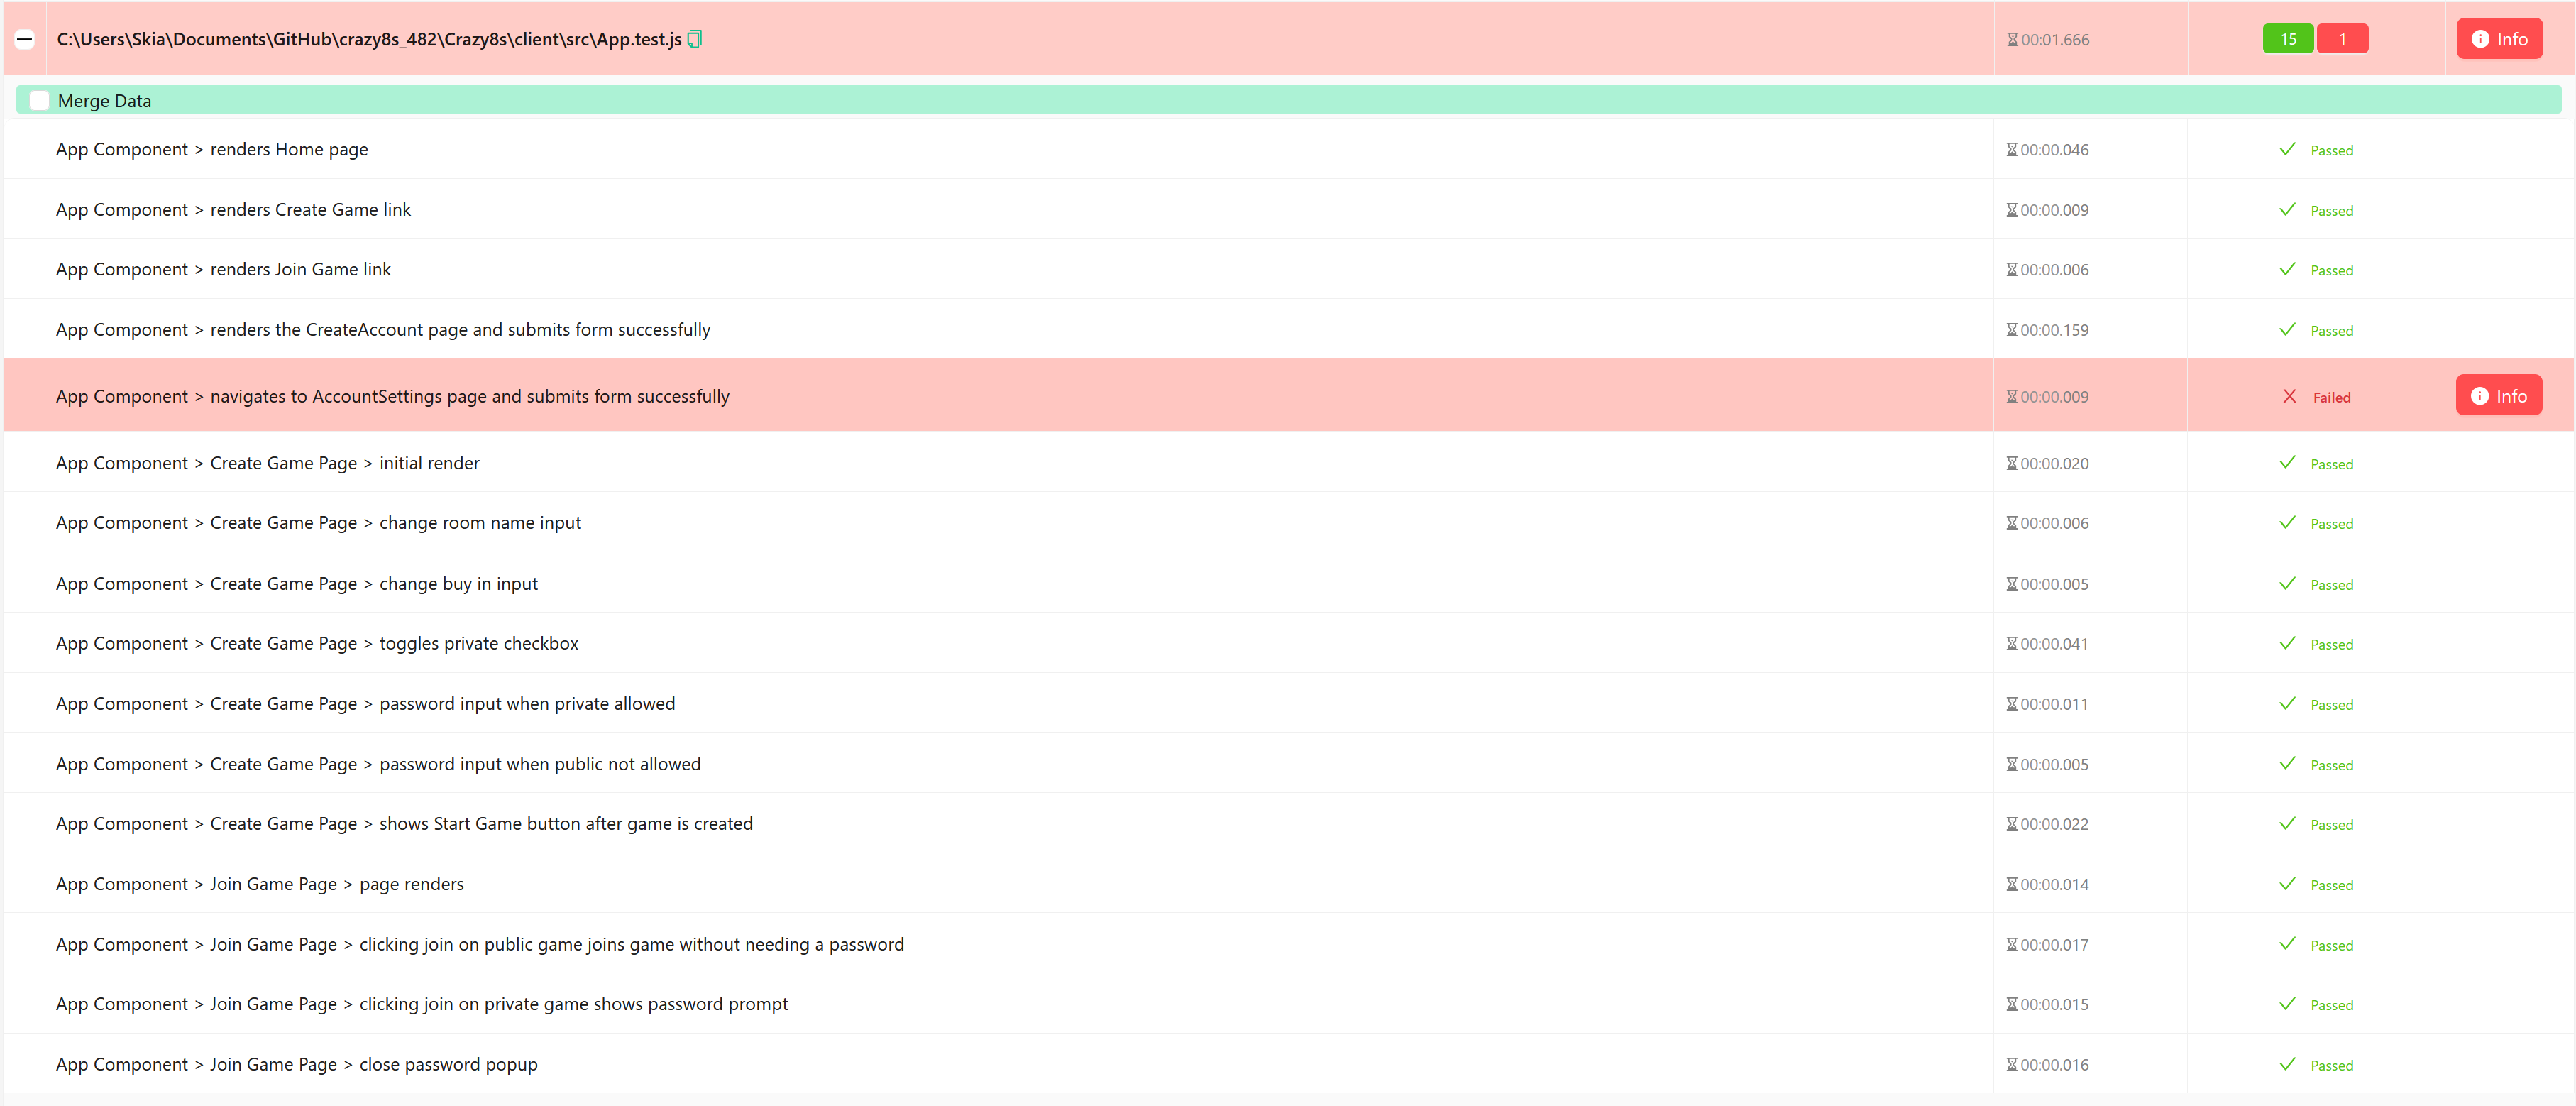
\includegraphics[width=\linewidth]{tests2_2.png}
\caption{\label{fig:testss2_2}The tests for the webpages using Jest.}
\end{figure}

\begin{figure}[h]
\centering
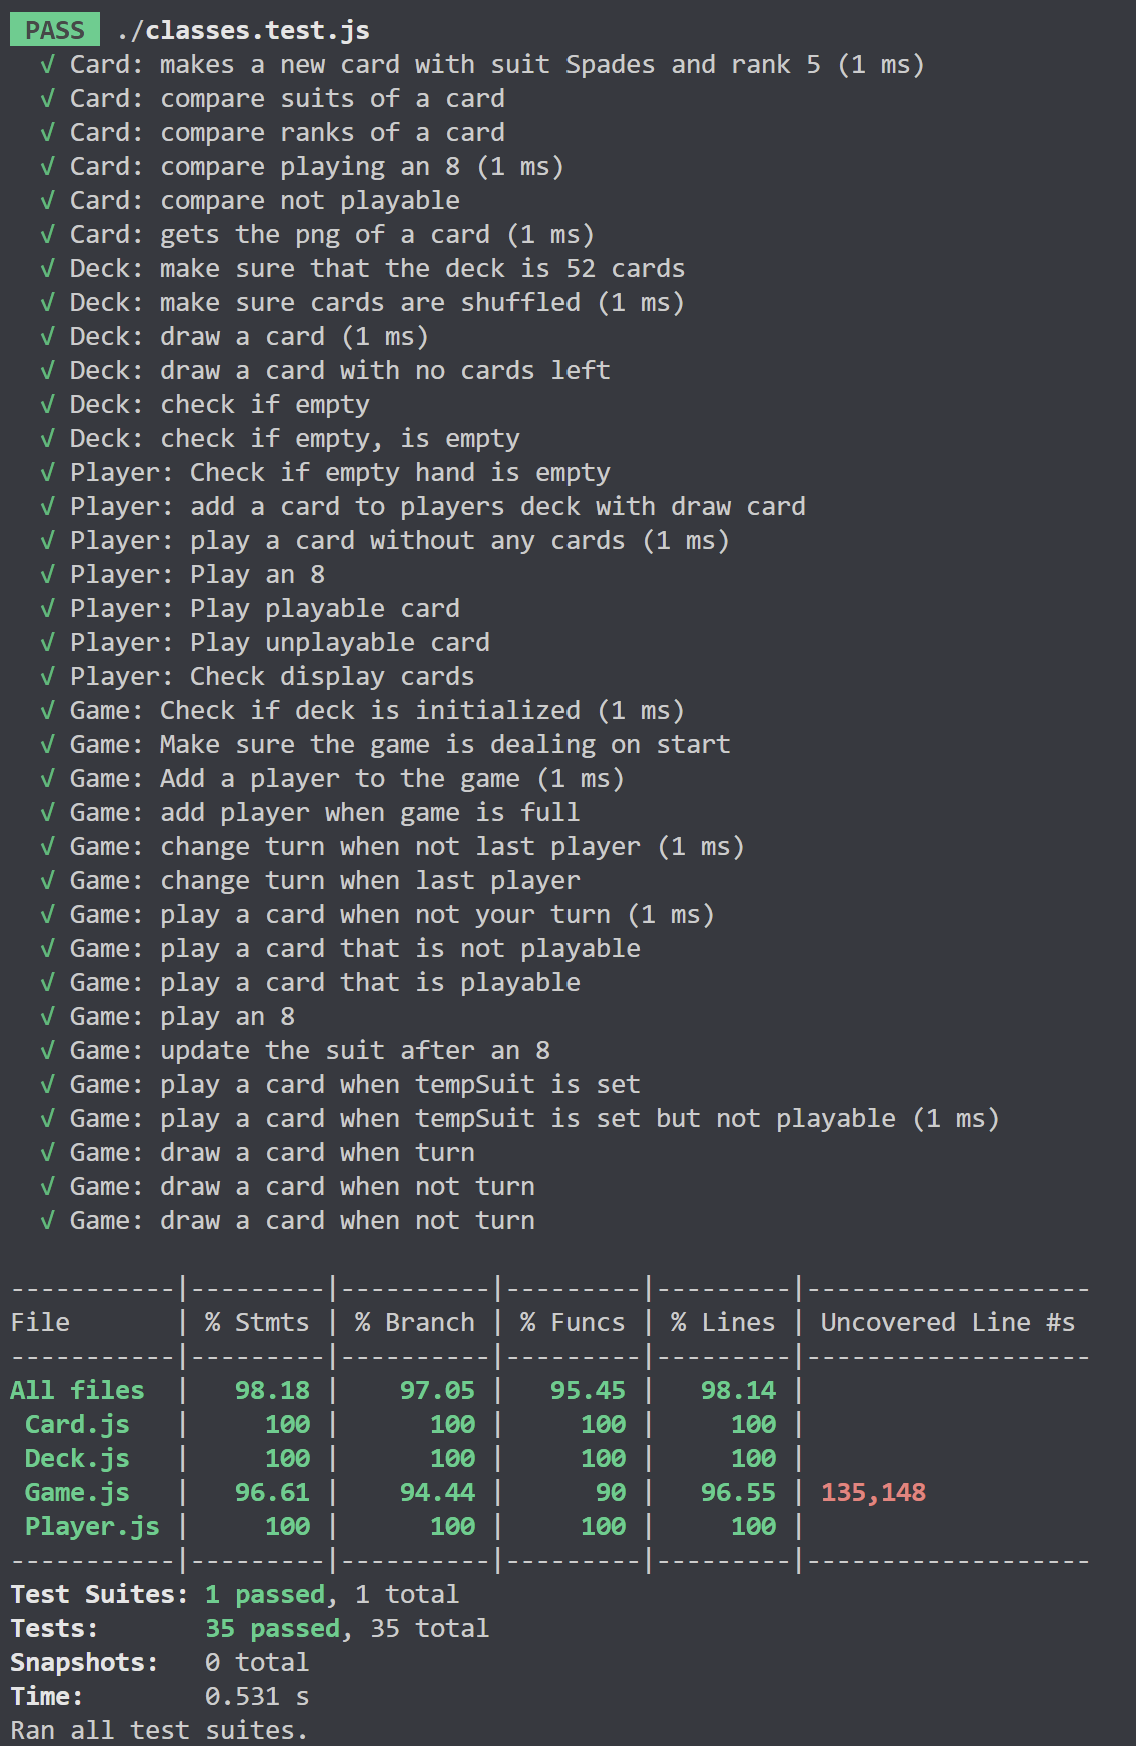
\includegraphics[width=\linewidth]{testss2_3.png}
\caption{\label{fig:testss2_3}The tests for the game functionality classes using Jest.}
\end{figure}

\begin{tcolorbox}[colback=blue!10, colframe=blue, boxrule=0.5mm, sharp corners=south]
\subsection{Sprint 3}

\subsubsection{Retrospective}
After the last sprint we were left with a few issues. The first being that most of the user stories were done very literally. An example of this is Play Card, which is completed, but didn't cover ending the game when someone won. By making some user story slices we hope to fix these gaps, and make sure the game runs smoothly. Testing was another issue we faced. We have found it difficult to mock react and socketio in Jest. This has hindered our branch coverage. We wish that we were able to figure it out sooner. So, this sprint we will put more emphasis on testing and make tests much earlier in the sprint.

\subsubsection{Changes and Slices}
For Sprint 3 we made several slices of user stories and a technical task. Firstly, we made a slice of "Play Card" called "End Game". This slice focused on ending the game when a player plays his or her last card. The second slice we made was from "Join Game". This slice we called "Connect Users to Game". This slice was primarily to track users through their games by adding a reference to the user session in the socket. Lastly, we made a technical task called "Improve UI" which was to make the UI more fluent and visually appealing.

\subsubsection{User Stories Attempted}
This sprint, we focused on fixing bugs, cleaning up the UI and finishing up the remaining user stories. Victoria took on: Improve UI, Tutorial, and Ads. Will finished some of his previous stories: Send Message, Add Friend, and Change Password. Jack took on: End Game, Connect Users to Game, Report and Read Player Report. Since Will was able to complete his stories quickly, he completed Report and Read Player Report while Jack focused on patching bugs and making the game runs smoothly.
\end{tcolorbox}

\begin{table}[h]
\centering
\begin{tabular}{|c|c|c|c|}
\hline
\textbf{Member} & \textbf{Stories Attempted} & \textbf{Story Points} & \textbf{Hours per Point} \\ \hline
Will     & 3 & 11  & 2 \\ \hline
Victoria & 3 & 9 & 3 \\ \hline
Jack     & 4 & 8 & 2 \\ \hline
Team    & 10 & 28 & 2.3 \\ \hline
\end{tabular}
\end{table}

\begin{tcolorbox}[colback=blue!10, colframe=blue, boxrule=0.5mm, sharp corners=south]
\subsubsection{Tests}

For sprint 3, we focused a lot more on testing, though it took a significant amount of time and we encountered a lot of issues with it. Our coverage is shown in \ref{fig:sprint3tests}. Branch coverage was around 40 percent.
\end{tcolorbox}

\begin{table}[h]
\centering
\begin{tabular}{|c|c|c|}
\hline
\textbf{} & \textbf{Area}     & \textbf{Coverage} \\ \hline
Jack      & Game Functions    & $\sim$80\%        \\ \hline
Victoria  & Main UI           & $\sim$50\%        \\ \hline
Will      & Account Functions & $\sim$30\%        \\ \hline
\end{tabular}
\end{table}

\begin{figure}[h]
\centering
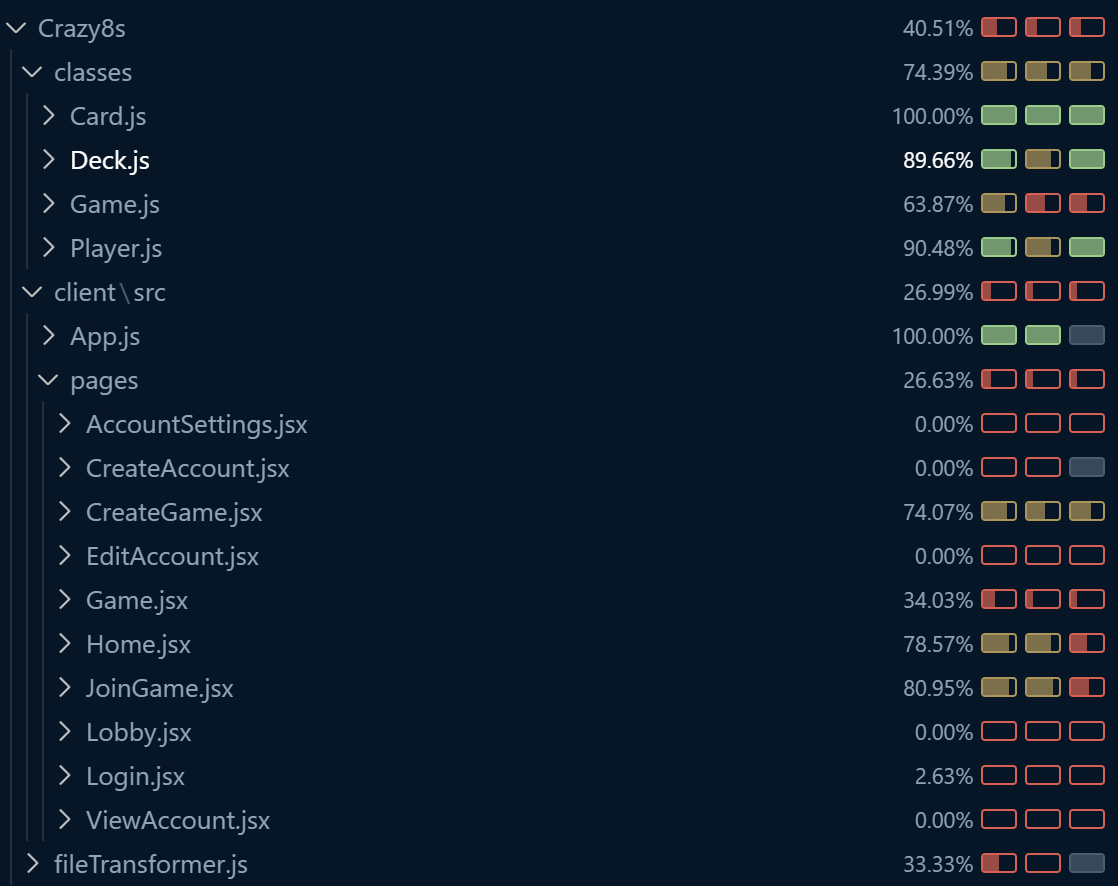
\includegraphics[width=\linewidth]{sprint3tests.png}
\caption{\label{fig:sprint3tests}The test coverage.}
\end{figure}

\begin{tcolorbox}[colback=blue!10, colframe=blue, boxrule=0.5mm, sharp corners=south]
\subsubsection{UML Class Diagram}
In our original UML we planned to have several more classes. We had a whole class dedicated to Users, UserStats and Admins. We also had a host class. At the time they seemed necessary. As we started to build the game, we realized that many of these classes were either useless or redundant. When it comes to Users, the database and user session handles all of that information. A host class didn't end up being necessary as there weren't any functions that we implemented that would be different. What we learned along the way is that socketio and as previously mentioned, express and firebase user sessions held a large chunk of the data. This led to a more condensed Class Diagram with few classes. The new diagram now only has four classes. These are just the game objects needed: Card, Player, Game, Deck. They interact much easier since socketio holds the persons Player. This way instead of searching for the player, we already have the object stored. Most functions use this by passing player as a parameter.
\end{tcolorbox}

\begin{figure}[h]
\centering
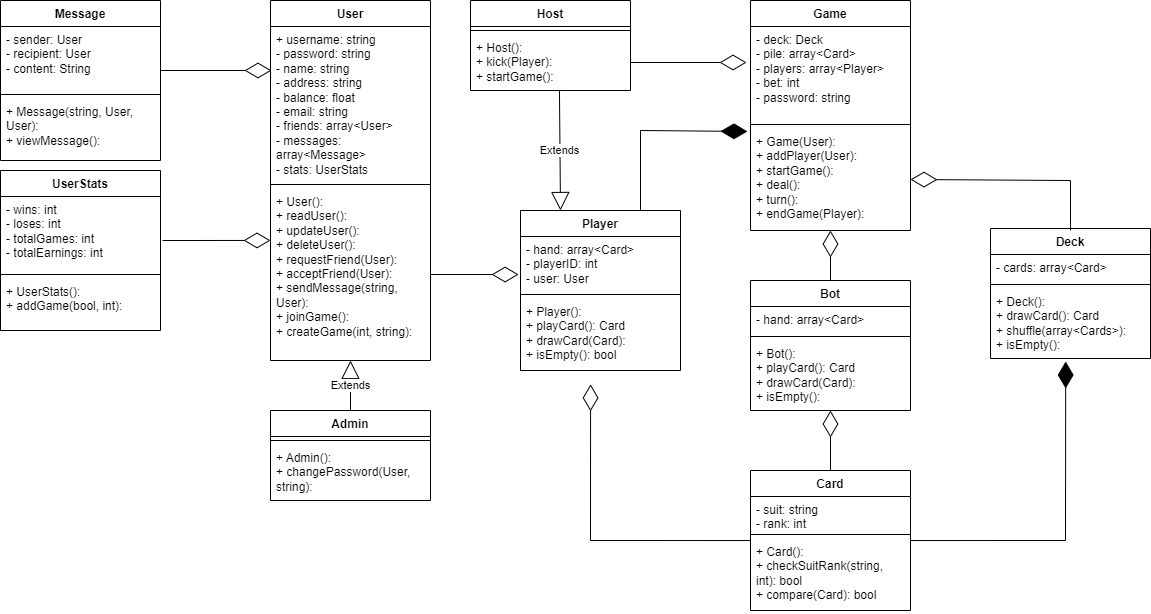
\includegraphics[width=\linewidth]{Crazy8sUML.png}
\caption{\label{fig:OldUML}Original UML Class Diagram.}
\end{figure}

\begin{figure}[h]
\centering
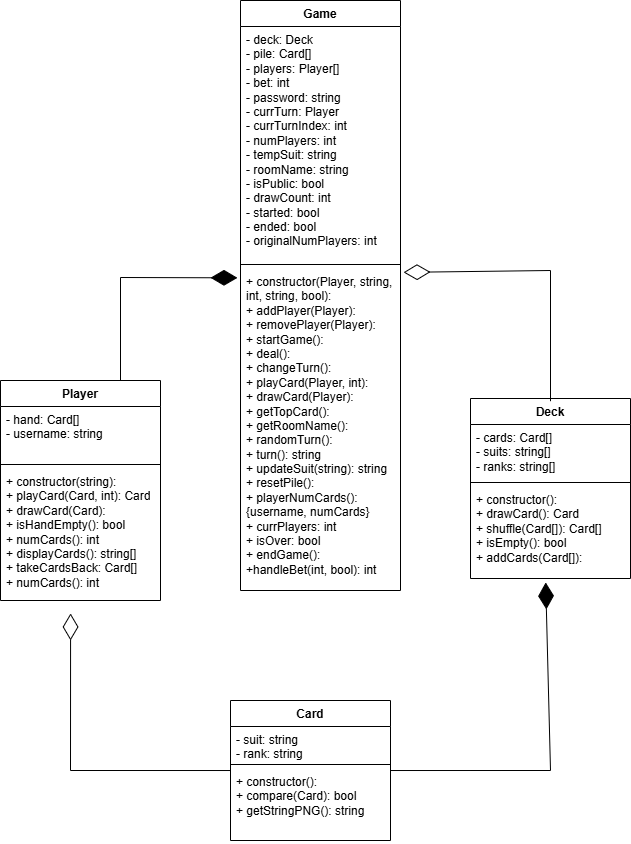
\includegraphics[width=\linewidth]{NewUML.png}
\caption{\label{fig:NewUML}Final UML Class Diagram.}
\end{figure}

\end{document}
